\documentclass[11pt,a4paper]{article}
\usepackage{fontspec}
\providecommand{\euro}{€}
\usepackage[french]{babel}
\usepackage[a4paper,margin=18mm,headheight=24pt]{geometry}
\usepackage{graphicx}
\usepackage[table]{xcolor}
\usepackage[most]{tcolorbox}
\usepackage{booktabs}
\usepackage{tabularx}
\usepackage{longtable}
\usepackage{xltabular}
\usepackage{array}
\usepackage[nobottomtitles*]{titlesec}
\usepackage{needspace}
\usepackage{fancyhdr}
\usepackage{fontawesome5}
\usepackage{etoolbox}
\usepackage[hidelinks]{hyperref}
\definecolor{sky}{HTML}{1C6DB4}
\definecolor{skyl}{HTML}{E6F0F8}
\definecolor{alert}{HTML}{B5382B}
\definecolor{alertl}{HTML}{FBE8EA}
\definecolor{summit}{HTML}{6B7A8F}
\definecolor{night}{HTML}{1B2A4A}
\definecolor{ink}{HTML}{1F2430}
\definecolor{or}{HTML}{B8860B}
\definecolor{orl}{HTML}{FBF3DC}
\AtBeginDocument{\color{ink}}
\titleformat{\section}{\Large\bfseries\sffamily\color{sky}}{}{0em}{}[{\vspace{1pt}\color{sky!35}\titlerule[1.1pt]}]
\titlespacing*{\section}{0pt}{14pt}{7pt}
\titleformat{\subsection}{\large\bfseries\sffamily\color{alert}}{}{0em}{}
\titlespacing*{\subsection}{0pt}{10pt}{4pt}
\pretocmd{\section}{\Needspace{10\baselineskip}}{}{}
\pretocmd{\subsection}{\Needspace{9\baselineskip}}{}{}
\widowpenalty=10000 \clubpenalty=10000 \raggedbottom
\setlength{\parindent}{0pt}\setlength{\parskip}{3pt}
\pagestyle{fancy}\fancyhf{}\renewcommand{\headrulewidth}{0.4pt}
\fancyhead[L]{\sffamily\small\color{night}\textbf{INVENTAIRE DE CAVE}}
\fancyhead[R]{\sffamily\small\color{summit}VEND\'EMIAIRE}
\fancyfoot[C]{\sffamily\small\color{summit}\thepage}
\newtcolorbox{cadrebox}[1]{enhanced,unbreakable,colback=skyl,colframe=sky,coltitle=white,fonttitle=\bfseries\sffamily\small,boxrule=0.9pt,arc=2.5pt,title={\faClipboardList~~#1}}
\newtcolorbox{warnbox}[1]{enhanced,breakable,colback=alertl,colframe=alert,coltitle=white,fonttitle=\bfseries\sffamily\small,boxrule=0.9pt,arc=2.5pt,title={\faExclamationTriangle~~#1}}
\BeforeBeginEnvironment{cadrebox}{\par\Needspace{9\baselineskip}}
\begin{document}
\begin{titlepage}\centering\vspace*{30mm}

\includegraphics[width=42mm]{logo.png}\\[12mm]
{\sffamily\bfseries\fontsize{28}{34}\selectfont\color{night} Inventaire de cave\par}\vspace{6mm}
{\sffamily\Large\color{sky} Rapport d'assurance et d'inventaire\par}\vspace{14mm}
{\large\color{summit} 26 octobre 2026\par}
\vfill
{\small\color{summit} Vend\'emiaire\par}
\end{titlepage}
\section{Résumé}
\begin{cadrebox}{Chiffres clés}
\begin{tabularx}{\linewidth}{@{}Xr@{}}
Vins & \textbf{6} \\
Bouteilles & \textbf{20} \\
Valeur retenue & \textbf{745,86~\euro{}} \\
dont bouteilles évaluées (valeur datée et sourcée) & 12 \\
dont bouteilles au prix d'achat & 8 \\
dont bouteilles sans valeur connue & 0 \\
\end{tabularx}
\end{cadrebox}
Méthode : pour chaque bouteille, la dernière valeur saisie pour ce vin dans ce format, avec sa date et sa source ; à défaut, le prix d'achat (indiqué comme tel, à la date d'achat) ; à défaut, « non évaluée ». Le niveau est lu sur l'échelle des maisons de ventes, avec ce qu'il signifie pour l'âge du vin (règles sourcées du dossier « Le vin »).

\subsection{Weingut Sonnenhang · Kabinett · Mosel · 2016}
\begin{minipage}[t]{\linewidth}
{\color{summit}Mosel · Moselle · Allemagne · Blanc}\par
Bouteilles : 4 — Valeur retenue : \textbf{76,40~\euro{}}
\end{minipage}\par\smallskip
{\footnotesize\begin{xltabular}{\linewidth}{@{}>{\raggedright\arraybackslash}p{0.22\linewidth}>{\raggedright\arraybackslash}X>{\raggedright\arraybackslash}p{0.17\linewidth}>{\raggedleft\arraybackslash}p{0.19\linewidth}@{}}
\toprule \textbf{Emplacement, format, code} & \textbf{Niveau, état, caisse, provenance} & \textbf{Achat} & \textbf{Valeur (date, source)} \\ \midrule \endhead
---\newline Bouteille\newline{\color{summit}\texttt{V50A25F4D1B}} & IN --- Dans le goulot (Excellent pour son âge)\newline Étiquette : Parfaite\newline Capsule : Intacte & 19,10~\euro{} · 18 janvier 2025 · Caviste & \textbf{19,10~\euro{}}\newline {\color{summit}prix d'achat, 18 janvier 2025} \\ \midrule[0.2pt]
---\newline Bouteille\newline{\color{summit}\texttt{V113D163BE0}} & IN --- Dans le goulot (Excellent pour son âge)\newline Étiquette : Parfaite\newline Capsule : Intacte & 19,10~\euro{} · 18 janvier 2025 · Caviste & \textbf{19,10~\euro{}}\newline {\color{summit}prix d'achat, 18 janvier 2025} \\ \midrule[0.2pt]
---\newline Bouteille\newline{\color{summit}\texttt{V2A1FF8C3C9}} & IN --- Dans le goulot (Excellent pour son âge)\newline Étiquette : Parfaite\newline Capsule : Intacte & 19,10~\euro{} · 18 janvier 2025 · Caviste & \textbf{19,10~\euro{}}\newline {\color{summit}prix d'achat, 18 janvier 2025} \\ \midrule[0.2pt]
---\newline Bouteille\newline{\color{summit}\texttt{V3851591093}} & IN --- Dans le goulot (Excellent pour son âge)\newline Étiquette : Parfaite\newline Capsule : Intacte & 19,10~\euro{} · 18 janvier 2025 · Caviste & \textbf{19,10~\euro{}}\newline {\color{summit}prix d'achat, 18 janvier 2025} \\ \midrule[0.2pt]
\bottomrule\end{xltabular}}
\subsection{Weingut Sonnenhang · Kabinett · Mosel · 2024}
\begin{minipage}[t]{\linewidth}
{\color{summit}Mosel · Moselle · Allemagne · Blanc}\par
Bouteilles : 4 — Valeur retenue : \textbf{140~\euro{}}
\end{minipage}\par\smallskip
{\footnotesize\begin{xltabular}{\linewidth}{@{}>{\raggedright\arraybackslash}p{0.22\linewidth}>{\raggedright\arraybackslash}X>{\raggedright\arraybackslash}p{0.17\linewidth}>{\raggedleft\arraybackslash}p{0.19\linewidth}@{}}
\toprule \textbf{Emplacement, format, code} & \textbf{Niveau, état, caisse, provenance} & \textbf{Achat} & \textbf{Valeur (date, source)} \\ \midrule \endhead
---\newline Bouteille\newline{\color{summit}\texttt{V5C328B1062}} & IN --- Dans le goulot (Excellent pour son âge)\newline Étiquette : Légèrement abîmée\newline Capsule : Intacte\newline Carton & 23,45~\euro{} · 11 avril 2018 · Foire aux vins & \textbf{35~\euro{}}\newline {\color{summit}estimation (démonstration), 26 septembre 2026} \\ \midrule[0.2pt]
---\newline Bouteille\newline{\color{summit}\texttt{V4B40BDD3FC}} & IN --- Dans le goulot (Excellent pour son âge)\newline Étiquette : Légèrement abîmée\newline Capsule : Intacte\newline Carton & 23,45~\euro{} · 11 avril 2018 · Foire aux vins & \textbf{35~\euro{}}\newline {\color{summit}estimation (démonstration), 26 septembre 2026} \\ \midrule[0.2pt]
---\newline Bouteille\newline{\color{summit}\texttt{V67AAAF8DD5}} & IN --- Dans le goulot (Excellent pour son âge)\newline Étiquette : Légèrement abîmée\newline Capsule : Intacte\newline Carton & 23,45~\euro{} · 11 avril 2018 · Foire aux vins & \textbf{35~\euro{}}\newline {\color{summit}estimation (démonstration), 26 septembre 2026} \\ \midrule[0.2pt]
---\newline Bouteille\newline{\color{summit}\texttt{V67256C8A1C}} & IN --- Dans le goulot (Excellent pour son âge)\newline Étiquette : Légèrement abîmée\newline Capsule : Intacte\newline Carton & 23,45~\euro{} · 11 avril 2018 · Foire aux vins & \textbf{35~\euro{}}\newline {\color{summit}estimation (démonstration), 26 septembre 2026} \\ \midrule[0.2pt]
\bottomrule\end{xltabular}}
\subsection{Bodegas Peña Alta · Reserva · Rioja · 2008}
\begin{minipage}[t]{0.22\linewidth}\vspace{0pt}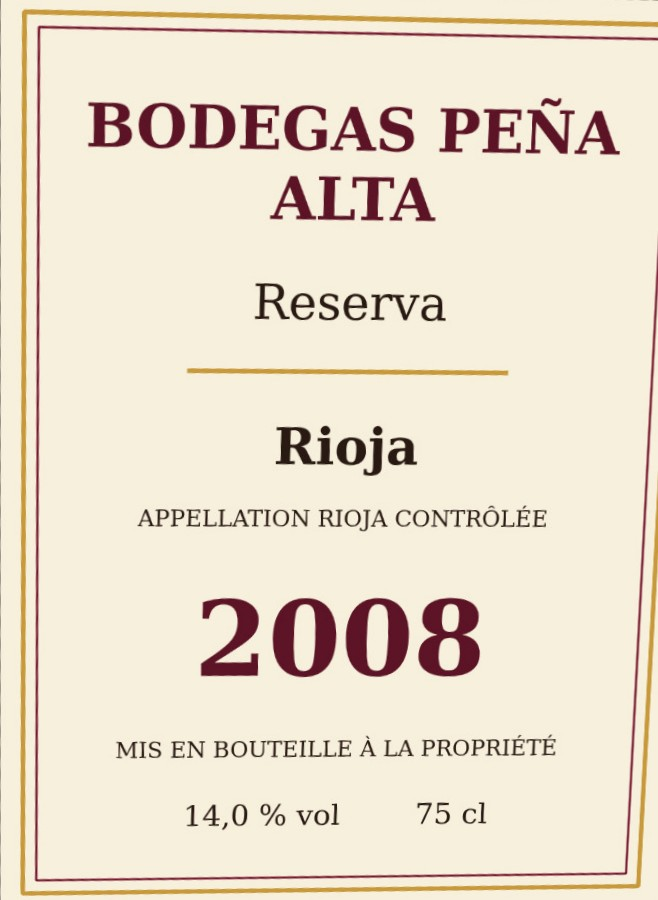
\includegraphics[width=\linewidth,height=42mm,keepaspectratio]{photo49.jpg}\end{minipage}\hfill\begin{minipage}[t]{0.75\linewidth}\vspace{0pt}
{\color{summit}Rioja · Rioja · Espagne · Rouge}\par
Bouteilles : 5 — Valeur retenue : \textbf{200~\euro{}}
\end{minipage}\par\smallskip
{\footnotesize\begin{xltabular}{\linewidth}{@{}>{\raggedright\arraybackslash}p{0.22\linewidth}>{\raggedright\arraybackslash}X>{\raggedright\arraybackslash}p{0.17\linewidth}>{\raggedleft\arraybackslash}p{0.19\linewidth}@{}}
\toprule \textbf{Emplacement, format, code} & \textbf{Niveau, état, caisse, provenance} & \textbf{Achat} & \textbf{Valeur (date, source)} \\ \midrule \endhead
Cave de la maison › Mur nord › Casier A (rangée 2, colonne 2)\newline Bouteille\newline{\color{summit}\texttt{VECFF20D6F6}} & IN --- Dans le goulot (Excellent pour son âge)\newline Étiquette : Légèrement abîmée\newline Capsule : Intacte\newline Carton & 24,70~\euro{} · 10 janvier 2021 · Au domaine & \textbf{40~\euro{}}\newline {\color{summit}estimation (démonstration), 26 septembre 2026} \\ \midrule[0.2pt]
Cave de la maison › Mur nord › Casier A (rangée 6, colonne 2)\newline Bouteille\newline{\color{summit}\texttt{VAC99A5767E}} & IN --- Dans le goulot (Excellent pour son âge)\newline Étiquette : Légèrement abîmée\newline Capsule : Intacte\newline Carton & 24,70~\euro{} · 10 janvier 2021 · Au domaine & \textbf{40~\euro{}}\newline {\color{summit}estimation (démonstration), 26 septembre 2026} \\ \midrule[0.2pt]
Cave de la maison › Mur nord › Casier A (rangée 4, colonne 5)\newline Bouteille\newline{\color{summit}\texttt{V7DA9DDB285}} & IN --- Dans le goulot (Excellent pour son âge)\newline Étiquette : Légèrement abîmée\newline Capsule : Intacte\newline Carton & 24,70~\euro{} · 10 janvier 2021 · Au domaine & \textbf{40~\euro{}}\newline {\color{summit}estimation (démonstration), 26 septembre 2026} \\ \midrule[0.2pt]
Cave de la maison › Mur nord › Casier A (rangée 2, colonne 3)\newline Bouteille\newline{\color{summit}\texttt{VC480E4F282}} & IN --- Dans le goulot (Excellent pour son âge)\newline Étiquette : Légèrement abîmée\newline Capsule : Intacte\newline Carton & 24,70~\euro{} · 10 janvier 2021 · Au domaine & \textbf{40~\euro{}}\newline {\color{summit}estimation (démonstration), 26 septembre 2026} \\ \midrule[0.2pt]
Cave de la maison › Mur nord › Casier A (rangée 1, colonne 9)\newline Bouteille\newline{\color{summit}\texttt{V1AB820A018}} & IN --- Dans le goulot (Excellent pour son âge)\newline Étiquette : Légèrement abîmée\newline Capsule : Intacte\newline Carton & 24,70~\euro{} · 10 janvier 2021 · Au domaine & \textbf{40~\euro{}}\newline {\color{summit}estimation (démonstration), 26 septembre 2026} \\ \midrule[0.2pt]
\bottomrule\end{xltabular}}
\subsection{Domaine Weinberg-Hoff · Grand cru Schlossberg · Alsace grand cru · 2006}
\begin{minipage}[t]{\linewidth}
{\color{summit}Alsace grand cru · Alsace · France · Blanc}\par
Bouteilles : 3 — Valeur retenue : \textbf{114~\euro{}}
\end{minipage}\par\smallskip
{\footnotesize\begin{xltabular}{\linewidth}{@{}>{\raggedright\arraybackslash}p{0.22\linewidth}>{\raggedright\arraybackslash}X>{\raggedright\arraybackslash}p{0.17\linewidth}>{\raggedleft\arraybackslash}p{0.19\linewidth}@{}}
\toprule \textbf{Emplacement, format, code} & \textbf{Niveau, état, caisse, provenance} & \textbf{Achat} & \textbf{Valeur (date, source)} \\ \midrule \endhead
Cave de la maison › Mur nord › Casier B (rangée 6, colonne 4)\newline Bouteille\newline{\color{summit}\texttt{V15C199CBAF}} & VTS --- Très haut d'épaule (Excellent pour son âge)\newline Étiquette : Parfaite\newline Capsule : Intacte\newline Carton & 31,19~\euro{} · 1er mai 2026 · Salon des vins & \textbf{38~\euro{}}\newline {\color{summit}estimation (démonstration), 26 septembre 2026} \\ \midrule[0.2pt]
Cave de la maison de montagne › Étagère › Rayonnage (rangée 2, colonne 5)\newline Bouteille\newline{\color{summit}\texttt{VB41EEEE927}} & VTS --- Très haut d'épaule (Excellent pour son âge)\newline Étiquette : Parfaite\newline Capsule : Intacte\newline Carton & 31,19~\euro{} · 1er mai 2026 · Salon des vins & \textbf{38~\euro{}}\newline {\color{summit}estimation (démonstration), 26 septembre 2026} \\ \midrule[0.2pt]
Cave de la maison › Mur nord › Casier A (rangée 3, colonne 9)\newline Bouteille\newline{\color{summit}\texttt{VEAC649AB04}} & VTS --- Très haut d'épaule (Excellent pour son âge)\newline Étiquette : Parfaite\newline Capsule : Intacte\newline Carton & 31,19~\euro{} · 1er mai 2026 · Salon des vins & \textbf{38~\euro{}}\newline {\color{summit}estimation (démonstration), 26 septembre 2026} \\ \midrule[0.2pt]
\bottomrule\end{xltabular}}
\subsection{Domaine du Grand Mûrier · Morgon · 2024}
\begin{minipage}[t]{0.22\linewidth}\vspace{0pt}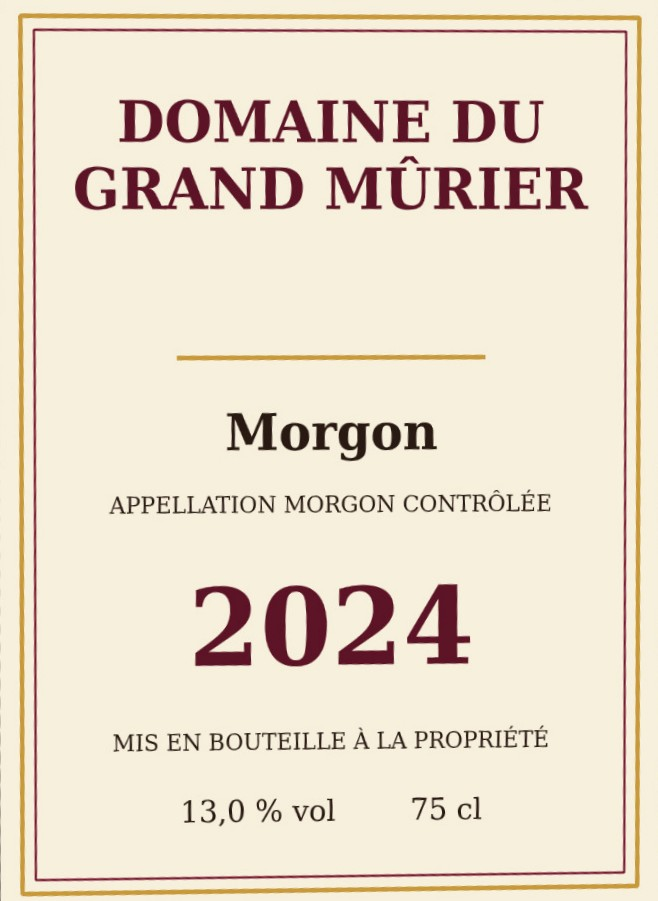
\includegraphics[width=\linewidth,height=42mm,keepaspectratio]{photo22.jpg}\end{minipage}\hfill\begin{minipage}[t]{0.75\linewidth}\vspace{0pt}
{\color{summit}Morgon · Beaujolais · France · Rouge}\par
Bouteilles : 2 — Valeur retenue : \textbf{37,06~\euro{}}
\end{minipage}\par\smallskip
{\footnotesize\begin{xltabular}{\linewidth}{@{}>{\raggedright\arraybackslash}p{0.22\linewidth}>{\raggedright\arraybackslash}X>{\raggedright\arraybackslash}p{0.17\linewidth}>{\raggedleft\arraybackslash}p{0.19\linewidth}@{}}
\toprule \textbf{Emplacement, format, code} & \textbf{Niveau, état, caisse, provenance} & \textbf{Achat} & \textbf{Valeur (date, source)} \\ \midrule \endhead
Cave de la maison › Armoire à vin › Clayette 2 (rangée 3, colonne 7)\newline Bouteille\newline{\color{summit}\texttt{V4ABAFCA208}} & IN --- Dans le goulot (Excellent pour son âge)\newline Étiquette : Parfaite\newline Capsule : Intacte & 18,53~\euro{} · 10 août 2019 · Salon des vins & \textbf{18,53~\euro{}}\newline {\color{summit}prix d'achat, 10 août 2019} \\ \midrule[0.2pt]
Cave de la maison › Armoire à vin › Clayette 1 (rangée 2, colonne 3)\newline Bouteille\newline{\color{summit}\texttt{V00F89D59CE}} & IN --- Dans le goulot (Excellent pour son âge)\newline Étiquette : Parfaite\newline Capsule : Intacte & 18,53~\euro{} · 10 août 2019 · Salon des vins & \textbf{18,53~\euro{}}\newline {\color{summit}prix d'achat, 10 août 2019} \\ \midrule[0.2pt]
\bottomrule\end{xltabular}}
\subsection{Château des Trois Chênes · Grand vin · Pauillac · 2016}
\begin{minipage}[t]{0.22\linewidth}\vspace{0pt}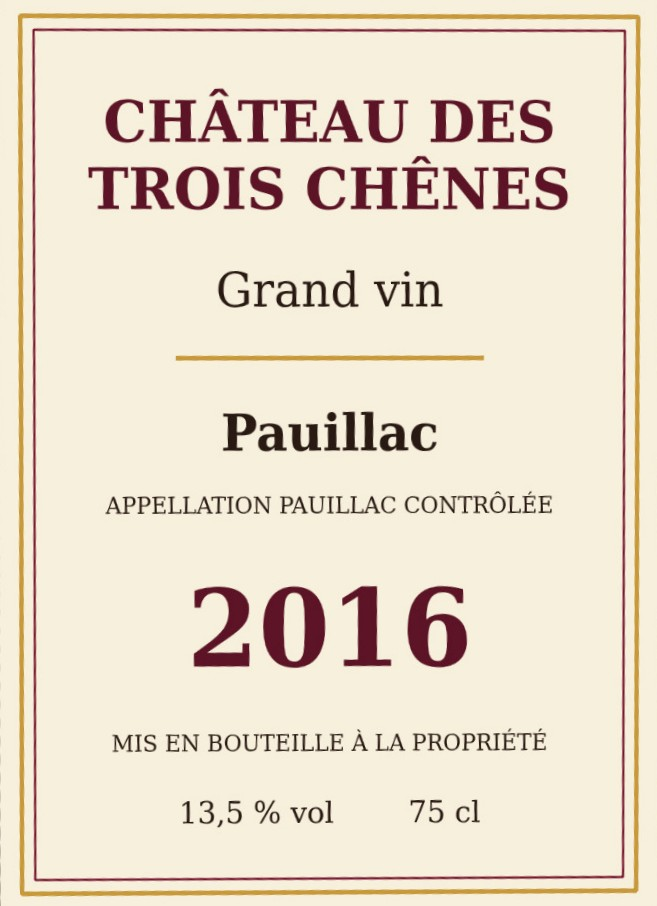
\includegraphics[width=\linewidth,height=42mm,keepaspectratio]{photo1.jpg}\end{minipage}\hfill\begin{minipage}[t]{0.75\linewidth}\vspace{0pt}
{\color{summit}Pauillac · Bordeaux · France · Rouge}\par
Bouteilles : 2 — Valeur retenue : \textbf{178,40~\euro{}}
\end{minipage}\par\smallskip
{\footnotesize\begin{xltabular}{\linewidth}{@{}>{\raggedright\arraybackslash}p{0.22\linewidth}>{\raggedright\arraybackslash}X>{\raggedright\arraybackslash}p{0.17\linewidth}>{\raggedleft\arraybackslash}p{0.19\linewidth}@{}}
\toprule \textbf{Emplacement, format, code} & \textbf{Niveau, état, caisse, provenance} & \textbf{Achat} & \textbf{Valeur (date, source)} \\ \midrule \endhead
Cave de la maison de montagne › Étagère › Rayonnage (rangée 4, colonne 5)\newline Bouteille\newline{\color{summit}\texttt{V85FCFBA971}} & IN --- Dans le goulot (Excellent pour son âge)\newline Étiquette : Parfaite\newline Capsule : Intacte\newline Carton & 89,20~\euro{} · 20 mai 2020 · Salon des vins & \textbf{89,20~\euro{}}\newline {\color{summit}prix d'achat, 20 mai 2020} \\ \midrule[0.2pt]
Cave de la maison › Mur nord › Casier A (rangée 5, colonne 7)\newline Bouteille\newline{\color{summit}\texttt{V08B3BA0F10}} & IN --- Dans le goulot (Excellent pour son âge)\newline Étiquette : Parfaite\newline Capsule : Intacte\newline Carton & 89,20~\euro{} · 20 mai 2020 · Salon des vins & \textbf{89,20~\euro{}}\newline {\color{summit}prix d'achat, 20 mai 2020} \\ \midrule[0.2pt]
\bottomrule\end{xltabular}}
\section{Attestation}
Je certifie que cet inventaire décrit les bouteilles présentes dans ma cave à la date du rapport.
\vspace{18mm}
\begin{tabularx}{\linewidth}{XX}
Fait à \dots{}\dots{}\dots{}\dots{}\dots{}\dots{}\dots{}, le \dots{}\dots{}\dots{}\dots{}\dots{} & Signature : \\ \end{tabularx}
\end{document}
